%%
%% Beginning of file 'sample.tex'
%%
%% Modified 2015 December
%%
%% This is a sample manuscript marked up using the
%% AASTeX v6.x LaTeX 2e macros.

%% AASTeX is now based on Alexey Vikhlinin's emulateapj.cls 
%% (Copyright 2000-2015).  See the classfile for details.
%%
%% AASTeX requires revtex4-1.cls (http://publish.aps.org/revtex4/) and
%% other external packages (latexsym, graphicx, amssymb, longtable, and epsf).
%% All of these external packages should already be present in the modern TeX 
%% distributions.  If not they can also be obtained at www.ctan.org.

%% The first piece of markup in an AASTeX v6.x document is the \documentclass
%% command. LaTeX will ignore any data that comes before this command. The 
%% documentclass can take an optional argument to modify the output style.
%% The command below calls the preprint style  which will produce a tightly 
%% typeset, one-column, single-spaced document.  It is the default and thus
%% does not need to be explicitly stated.
%%

%% using aastex version 6
\documentclass[onecolumn]{aastex6}
\usepackage{subfigure}
\usepackage{amsmath}
\usepackage{listings}
\usepackage{color}
 
\definecolor{codegreen}{rgb}{0,0.6,0}
\definecolor{codegray}{rgb}{0.5,0.5,0.5}
\definecolor{codepurple}{rgb}{0.58,0,0.82}
\definecolor{backcolour}{rgb}{0.95,0.95,0.92}
 
\lstdefinestyle{mystyle}{
    backgroundcolor=\color{backcolour},   
    commentstyle=\color{codegreen},
    keywordstyle=\color{magenta},
    numberstyle=\tiny\color{codegray},
    stringstyle=\color{codepurple},
    basicstyle=\footnotesize,
    breakatwhitespace=false,         
    breaklines=true,                 
    captionpos=b,                    
    keepspaces=true,                 
    numbers=left,                    
    numbersep=5pt,                  
    showspaces=false,                
    showstringspaces=false,
    showtabs=false,                  
    tabsize=2
}
 
\lstset{style=mystyle}


%% The other main article choice is a tightly typeset, two-column article
%% that more closely resembles the final typeset pdf article.
%%
%% \documentclass[twocolumn]{aastex6}
%% 
%% There are other optional arguments one can envoke to allow other 
%% actions. 
%%
% These are the available options:
%   manuscript	: onecolumn, doublespace, 12pt fonts
%   preprint	: onecolumn, single space, 10pt fonts
%   preprint2	: twocolumn, single space, 10pt fonts
%   twocolumn	: a two column article. Probably not needed, but here just in case.
%   onecolumn	: a one column article; default option.
%   twocolappendix: make 2 column appendix
%   onecolappendix: make 1 column appendix is the default. 
%   astrosymb	: Loads Astrosymb font and define \astrocommands. 
%   tighten	: Makes baselineskip slightly smaller
%   times	: uses times font instead of the default
%   linenumbers	: turn on lineno package.
%   trackchanges : required to see the revision mark up and print output
%   numberedappendix: Labels appendix sections A, B, ... This is the default.
%   appendixfloats: Needed. Resets figure and table counters to zero

%% these can be used in any combination, e.g.
%%
%% \documentclass[twocolumn,twocolappendix,linenumbers,trackchanges]{aastex6}

%% If you want to create your own macros, you can do so
%% using \newcommand. Your macros should appear before
%% the \begin{document} command.
%%
\newcommand{\vdag}{(v)^\dagger}
\newcommand\aastex{AAS\TeX}
\newcommand\latex{La\TeX}

%% AASTeX 6.0 supports the ability to suppress the names and affiliations
%% of some authors and displaying them under a "collaboration" banner to
%% minimize the amount of author information that to be printed.  This 
%% should be reserved for articles with an extreme number of authors.
%%
%% Mark up commands to limit the number of authors on the front page.
\AuthorCallLimit=2
%% Will only show Schwarz & Muench since Schwarz and Muench
%% are in the same \author call. 
\fullcollaborationName{The Friends of AASTeX Collaboration}
%% will print the collaboration text after the shortened author list.
%% These commands have to COME BEFORE the \author calls.
%%
%% Note that all of these author will be shown in the published article.
%% This feature is meant to be used prior to acceptance to make the
%% front end of a long author article more manageable.
%% Use \allauthors at the manuscript end to show the full author list.

%% The following command can be used to set the latex table counters.  It
%% is needed in this document because it uses a mix of latex tabular and
%% AASTeX deluxetables.  In general it should not be needed.
%\setcounter{table}{1}

%%%%%%%%%%%%%%%%%%%%%%%%%%%%%%%%%%%%%%%%%%%%%%%%%%%%%%%%%%%%%%%%%%%%%%%%%%%%%%%%
%%
%% The following commented section outlines numerous optional output that
%% can be displayed in the front matter or as running meta-data.
%%
%% You can insert a short comment on the title page using the command below.
%% \slugcomment{Not to appear in Nonlearned J., 45.}
%%
%% If you wish, you may supply running head information, although
%% this information may be modified by the editorial offices.
%%\shorttitle{\aastex sample article}
%%\shortauthors{Schwarz et al.}
%%
%% You can add a light gray and diagonal water-mark to the first page 
%% with this command:
%% \watermark{text}
%% where "text", e.g. DRAFT, is the text to appear.  If the text is 
%% long you can control the water-mark size with:
%% \setwatermarkfontsize{dimension}
%% where dimension is any recognized LaTeX dimension, e.g. pt, in, etc.
%%
%%%%%%%%%%%%%%%%%%%%%%%%%%%%%%%%%%%%%%%%%%%%%%%%%%%%%%%%%%%%%%%%%%%%%%%%%%%%%%%%

%% This is the end of the preamble.  Indicate the beginning of the
%% paper itself with \begin{document}.

\begin{document}

%% LaTeX will automatically break titles if they run longer than
%% one line. However, you may use \\ to force a line break if
%% you desire.

\title{HW 04: Line Broadening}

%% Use \author, \affil, plus the \and command to format author and affiliation 
%% information.  If done correctly the peer review system will be able to
%% automatically put the author and affiliation information from the manuscript
%% and save the corresponding author the trouble of entering it by hand.
%%
%% The \affil should be used to document primary affiliations and the
%% \altaffil should be used for secondary affiliations, titles, or email.

%% Authors with the same affiliation can be grouped in a single
%% \author and \affil call.
\author{Bryan Yamashiro\altaffilmark{1}}
\affil{University of Hawaii at Manoa \\
2500 Campus Road \\
Honolulu, HI 96822}


%% Use the \and command so offset the last author.

%% Notice that each of these authors has alternate affiliations, which
%% are identified by the \altaffilmark after each name.  Specify alternate
%% affiliation information with \altaffiltext, with one command per each
%% affiliation.

%\altaffiltext{1}{A cool dude}
%\altaffiltext{2}{Another cool dude}


%% From the front matter, we move on to the body of the paper.
%% Sections are demarcated by \section and \subsection, respectively.
%% Observe the use of the LaTeX \label
%% command after the \subsection to give a symbolic KEY to the
%% subsection for cross-referencing in a \ref command.
%% You can use LaTeX's \ref and \label commands to keep track of
%% cross-references to sections, equations, tables, and figures.
%% That way, if you change the order of any elements, LaTeX will
%% automatically renumber them.

%% We recommend that authors also use the natbib \citep
%% and \citet commands to identify citations.  The citations are
%% tied to the reference list via symbolic KEYs. The KEY corresponds
%% to the KEY in the \bibitem in the reference list below. 

\section{Natural Broadening}

The equation used to generate the Lorentz profile is provided in equation\,\ref{lorentz}. The profile is shown in figure\,\ref{broadening}\,(left), with a green line to indicate the half maximum intensity. Based on the figure, the full width at half maximum is approximately $2.5\times10^{-4}\,\AA$, which agrees with $\Gamma/2\pi$.

\begin{equation}
\phi_\nu = \frac{\Gamma/4\pi^2}{(\nu-\nu_0)^2 + (\Gamma/4\pi)^2}
\label{lorentz}
\end{equation}

\begin{figure*}[ht]
  \centering
  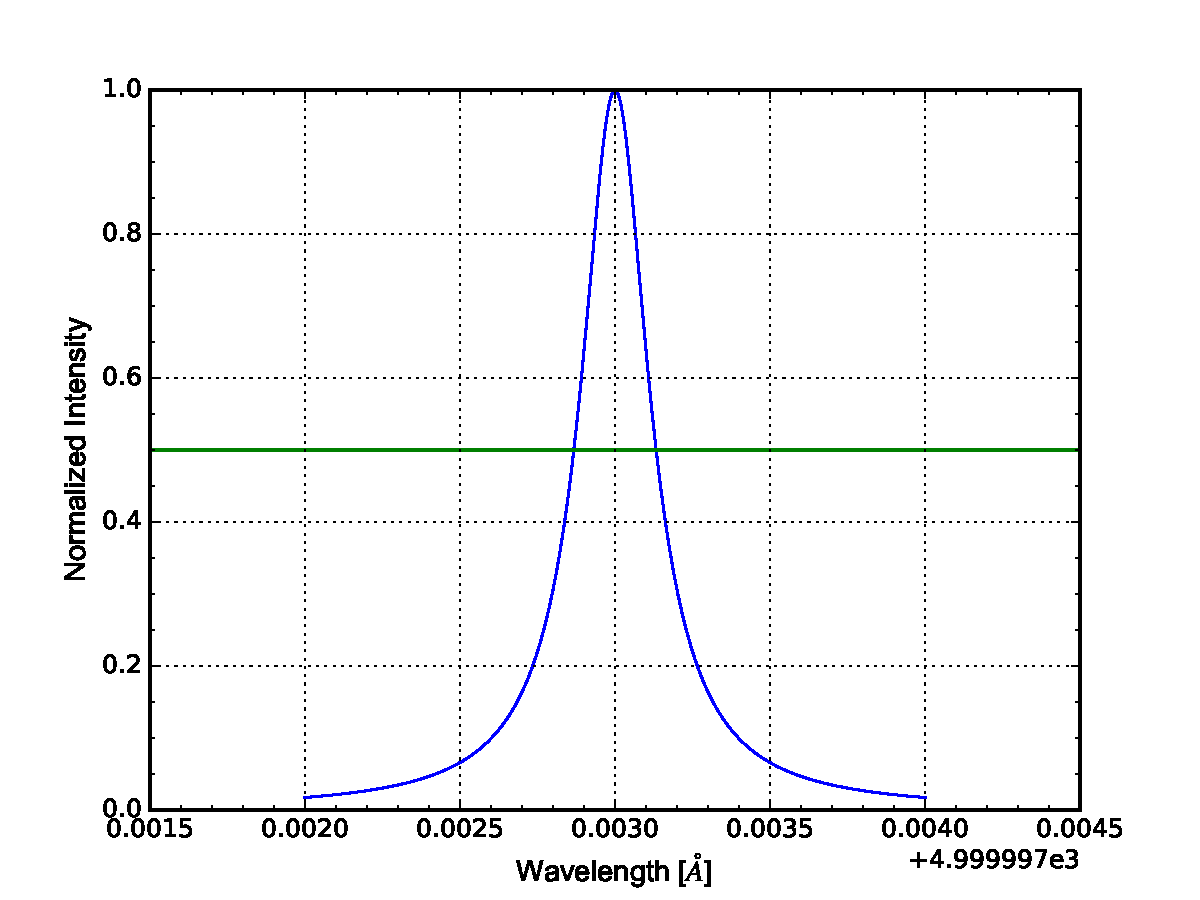
\includegraphics[scale=0.3]{nat1.pdf}%\quad
  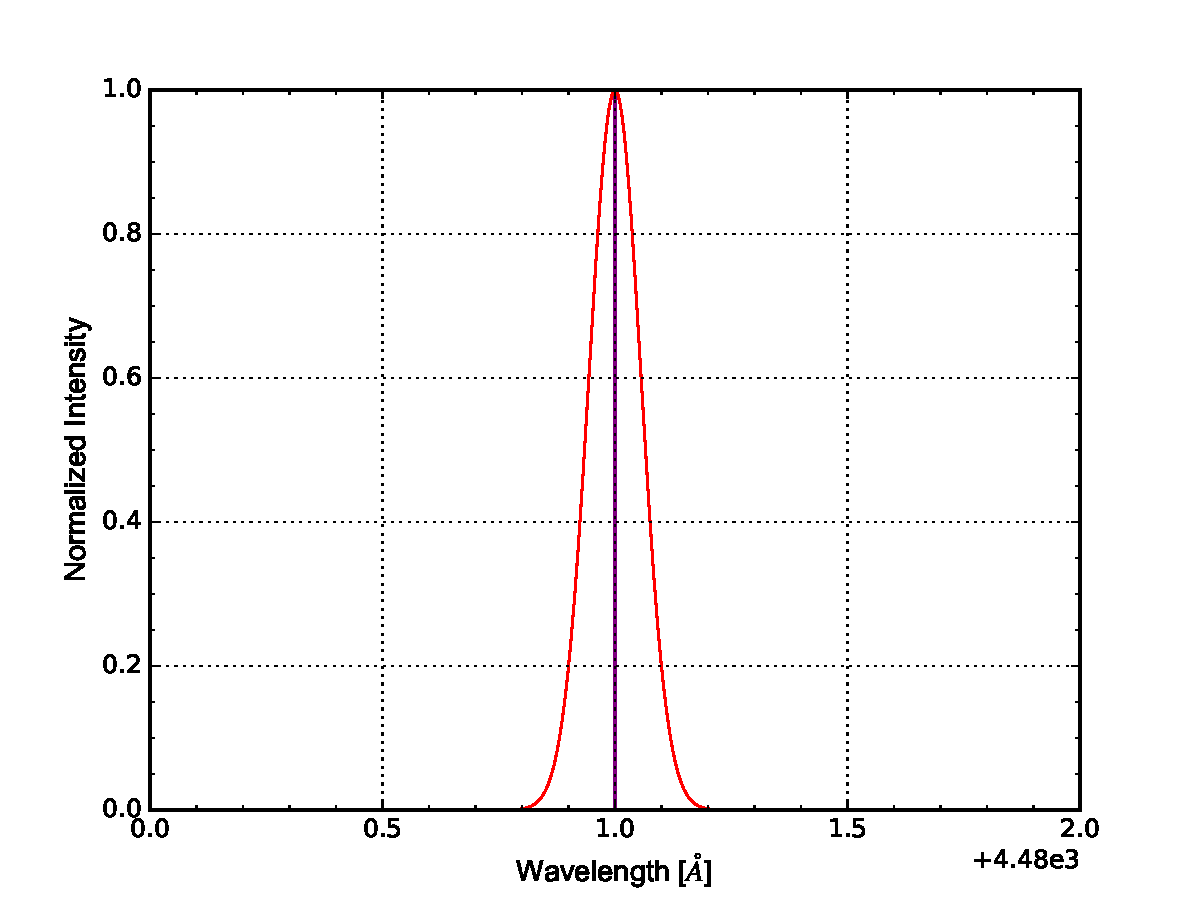
\includegraphics[scale=0.3]{withoutshift.pdf}%\quad
  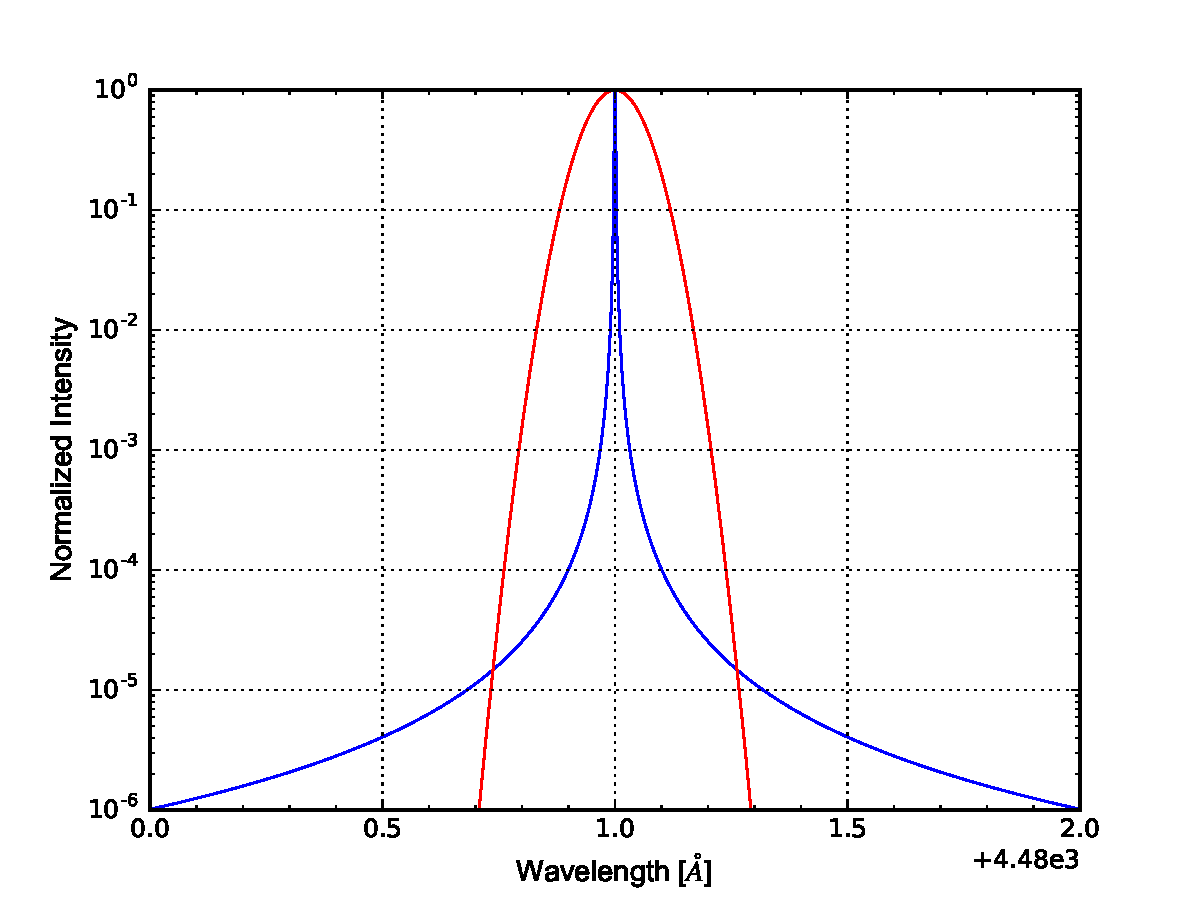
\includegraphics[scale=0.3]{dopper.pdf} \\%\quad

  \caption{Profiles for Lorentz\,(left), Doppler\,(middle), and a combination of the two\,(right).}
  \label{broadening}
\end{figure*}

\section{Doppler Broadening}

The equation used to generate the Doppler broadening is provided in equation\,\ref{doppler}. The profile is shown in figure\,\ref{broadening}\,(middle). The V$_{th}$ and the $\Delta\lambda_D^2$ found for the Mg II line at 4481\,\AA were 2.6322\,km/s and 0.0787\,\AA, respectively. The normalized intensity when inputting $\lambda = \lambda_0 + \Delta\lambda_D^2$ in equation\,\ref{doppler}, was 0.3679. When both the Lorentz and Doppler profiles are compared, figure\,\ref{broadening}\,(right), the wavelength at which the Lorentz profile is greater than the Doppler is at approximately 4481.27\,\AA. 

\begin{equation}
exp(-\frac{(\lambda-\lambda_0)^2}{\Delta\lambda_D^2})
\label{doppler}
\end{equation}

%\acknowledgments

\section{Rotation}
The stellar parameters in table\,\ref{spectable}, used for this section were found at the Caltech "Encyclopedia of Astronomy and Astrophysics"\,(\url{http://www.astro.caltech.edu/~george/ay20/eaa-stellarmasses.pdf}). The highest escape velocities were from spectral class O, and in general, the higher spectral classes. Rotational velocities of the main sequence objects were found in the "Allen-Astrophysical Quantities" reference, and consisted of the vsin(i) parameters. The maximum rotational broadening were found using the vsin(i) parameters against the speed of light. For a B-type star, the maximum rotational broadening is approximately 6004\,\AA
\\
\indent It cannot be an H-line because of pressure broadening\,(Stark). The Stark broadening in particular is not sensitive to rotational broadening, therefore it must be a metal line or else Stark broadening dominates the profile.


\begin{deluxetable}{cccccc}
\tablecaption{Stellar Parameters.}
\tablecolumns{6}
\tablenum{1}
\tablewidth{0pt}
\tablehead{
\colhead{Spectral Class}  & \colhead{Mass}& \colhead{Radius}& \colhead{Escape Velocity}& \colhead{v$_e$sin(i)}  & \colhead{Max Rotational Broadening}\\
\colhead{} & \colhead{[M$_\odot$]}& \colhead{[R$_\odot$]}& \colhead{[km/s]}& \colhead{[km/s]}& \colhead{[\AA]} }
\centering
\startdata
O4\,V       &   60    &  10       &  1513.187402 &    140     &4669.897333 \\
B5\,V       &   5    &  2.7       &  840.6596678 &    180     &6004.153714 \\
A2\,III     &   2.5    & 3.8      &  501.0664191 &   160      &5337.025523 \\
F5\,V       &    1.25   & 1.2     &  630.4947509 &   60       &2001.384571 \\
G8\,V       &   1    &   1.2    &   563.931649  &   20      &667.1281904
\enddata  
%\tablenotetext{a}{At exposure start.}
\tablecomments{Stellar parameters found from derivations and catalogs.}
\label{spectable}
\end{deluxetable}

\vspace{5mm}





%% Appendix material should be preceded with a single \appendix command.
%% There should be a \section command for each appendix. Mark appendix
%% subsections with the same markup you use in the main body of the paper.

%% Each Appendix (indicated with \section) will be lettered A, B, C, etc.
%% The equation counter will reset when it encounters the \appendix
%% command and will number appendix equations (A1), (A2), etc.


%% The reference list follows the main body and any appendices.
%% Use LaTeX's thebibliography environment to mark up your reference list.
%% Note \begin{thebibliography} is followed by an empty set of
%% curly braces.  If you forget this, LaTeX will generate the error
%% "Perhaps a missing \item?".
%%
%% thebibliography produces citations in the text using \bibitem-\cite
%% cross-referencing. Each reference is preceded by a
%% \bibitem command that defines in curly braces the KEY that corresponds
%% to the KEY in the \cite commands (see the first section above).
%% Make sure that you provide a unique KEY for every \bibitem or else the
%% paper will not LaTeX. The square brackets should contain
%% the citation text that LaTeX will insert in
%% place of the \cite commands.

%% We have used macros to produce journal name abbreviations.
%% \aastex provides a number of these for the more frequently-cited journals.
%% See the Author Guide for a list of them.

%% Note that the style of the \bibitem labels (in []) is slightly
%% different from previous examples.  The natbib system solves a host
%% of citation expression problems, but it is necessary to clearly
%% delimit the year from the author name used in the citation.
%% See the natbib documentation for more details and options.


\end{document}

%% End of file `sample.tex'.
